\documentclass[11pt]{article}
\usepackage{microtype}
\usepackage{graphicx}
\usepackage{wrapfig}
\usepackage{url}
\usepackage{wrapfig}
\usepackage{color}
\usepackage{marvosym}
\usepackage{enumerate}
\usepackage{subfigure}
\usepackage{tikz}
\usetikzlibrary{arrows}
\usetikzlibrary{shapes}
\usepackage{pgf}
\usepackage[fleqn]{amsmath}
\DeclareMathOperator*{\argmax}{arg\,max}
\DeclareMathOperator*{\argmin}{arg\,min}
\usepackage{amssymb}
\usepackage{hyperref}
\usepackage[many]{tcolorbox}
\usepackage{lipsum}
\usepackage{float}
\usepackage{trimclip}
\usepackage{listings}
\usepackage{environ}% http://ctan.org/pkg/environ
\usepackage{wasysym}
\usepackage{array}


\oddsidemargin 0mm
\evensidemargin 5mm
\topmargin -20mm
\textheight 240mm
\textwidth 160mm

\newcommand{\vwi}{{\bf w}_i}
\newcommand{\vw}{{\bf w}}
\newcommand{\vx}{{\bf x}}
\newcommand{\vy}{{\bf y}}
\newcommand{\vxi}{{\bf x}_i}
\newcommand{\yi}{y_i}
\newcommand{\vxj}{{\bf x}_j}
\newcommand{\vxn}{{\bf x}_n}
\newcommand{\yj}{y_j}
\newcommand{\ai}{\alpha_i}
\newcommand{\aj}{\alpha_j}
\newcommand{\X}{{\bf X}}
\newcommand{\Y}{{\bf Y}}
\newcommand{\vz}{{\bf z}}
\newcommand{\msigma}{{\bf \Sigma}}
\newcommand{\vmu}{{\bf \mu}}
\newcommand{\vmuk}{{\bf \mu}_k}
\newcommand{\msigmak}{{\bf \Sigma}_k}
\newcommand{\vmuj}{{\bf \mu}_j}
\newcommand{\msigmaj}{{\bf \Sigma}_j}
\newcommand{\pij}{\pi_j}
\newcommand{\pik}{\pi_k}
\newcommand{\D}{\mathcal{D}}
\newcommand{\el}{\mathcal{L}}
\newcommand{\N}{\mathcal{N}}
\newcommand{\vxij}{{\bf x}_{ij}}
\newcommand{\vt}{{\bf t}}
\newcommand{\yh}{\hat{y}}
\newcommand{\code}[1]{{\footnotesize \tt #1}}
\newcommand{\alphai}{\alpha_i}
\newcommand{\defeq}{\overset{\text{def}}{=}}
\renewcommand{\vec}[1]{\mathbf{#1}}
\newcommand{\nodesize}{0.8}
\newcommand{\ci}{\mathrel{\text{\scalebox{1.07}{$\perp\mkern-10mu\perp$}}}}

\bgroup
\def\arraystretch{1.5}
\newcolumntype{x}[1]{>{\centering\arraybackslash\hspace{0pt}}p{#1}}
\newcolumntype{z}[1]{>{\centering\arraybackslash}m{#1}}

%Arguments are 1 - height, 2 - box title
\newtcolorbox{textanswerbox}[2]{%
 width=\textwidth,colback=white,colframe=blue!30!black,floatplacement=H,height=#1,title=#2,clip lower=true,before upper={\parindent0em}}

 \newtcolorbox{eqanswerbox}[1]{%
 width=#1,colback=white,colframe=black,floatplacement=H,height=3em,sharp corners=all,clip lower=true,before upper={\parindent0em}}

 %Arguments are 1 - height, 2 - box title
 \NewEnviron{answertext}[2]{
        \noindent
        \marginbox*{0pt 10pt}{
        \clipbox{0pt 0pt 0pt 0pt}{
        \begin{textanswerbox}{#1}{#2}
        \BODY
        \end{textanswerbox}
        }
        }
}

%Arguments are 1 - height, 2 - box title, 3 - column definition
 \NewEnviron{answertable}[3]{
        \noindent
        \marginbox*{0pt 10pt}{
        \clipbox{0pt 0pt 0pt 0pt}{
        \begin{textanswerbox}{#1}{#2}
                \vspace{-0.5cm}
                        \begin{table}[H]
                        \centering
                        \begin{tabular}{#3}
                                \BODY
                        \end{tabular}
                        \end{table}
        \end{textanswerbox}
        }
        }
}

 %Arguments are 1 - height, 2 - box title, 3 - title, 4- equation label, 5 - equation box width
 \NewEnviron{answerequation}[5]{
        \noindent
        \marginbox*{0pt 10pt}{
        \clipbox{0pt 0pt 0pt 0pt}{
        \begin{textanswerbox}{#1}{#2}
                \vspace{-0.5cm}
                        \begin{table}[H]
                        \centering
                \renewcommand{\arraystretch}{0.5}% Tighter

                        \begin{tabular}{#3}
                                #4 =	&
                        \clipbox{0pt 0pt 0pt 0pt}{

                        \begin{eqanswerbox}{#5}
                                $\BODY$
                        \end{eqanswerbox}
                        } \\
                        \end{tabular}
                        \end{table}

        \end{textanswerbox}
        }
        }
}

 %Arguments are 1 - height, 2 - box title
 \NewEnviron{answerderivation}[2]{
        \noindent
        \marginbox*{0pt 10pt}{
        \clipbox{0pt 0pt 0pt 0pt}{
        \begin{textanswerbox}{#1}{#2}
        \BODY
        \end{textanswerbox}
        }
        }
}

\newcommand{\Checked}{{\LARGE \XBox}}%
\newcommand{\Unchecked}{{\LARGE \Square}}%
\newcommand{\TextRequired}{{\textbf{Place Answer Here}}}%
\newcommand{\EquationRequired}{\textbf{Type Equation Here}}%


\newcommand{\answertextheight}{5cm}
\newcommand{\answertableheight}{4cm}
\newcommand{\answerequationheight}{2.5cm}
\newcommand{\answerderivationheight}{14cm}

\newcounter{QuestionCounter}
\newcounter{SubQuestionCounter}[QuestionCounter]
\setcounter{SubQuestionCounter}{1}

\newcommand{\subquestiontitle}{Question \theQuestionCounter.\theSubQuestionCounter~}
\newcommand{\newquestion}{\stepcounter{QuestionCounter}\setcounter{SubQuestionCounter}{1}\newpage}
\newcommand{\newsubquestion}{\stepcounter{SubQuestionCounter}}

\DeclareMathOperator{\rank}{rank}
\DeclareMathOperator{\indices}{indices}
\DeclareMathOperator{\Bernoulli}{Bernoulli}
\DeclareMathOperator{\Bin}{Bin}
\DeclareMathOperator{\E}{E}
\DeclareMathOperator{\Var}{Var}
\DeclareMathOperator{\Cov}{Cov}

\lstset{language=[LaTeX]TeX,basicstyle=\ttfamily\bf}

\pagestyle{myheadings}
\markboth{Homework 4}{Fall 2024 CS 475/675 Machine Learning: Homework 4}

\title{CS 475 Machine Learning: Homework 4 Analytical \\
(70 points)\\
\Large{Assigned: Friday, November 01, 2024} \\
\Large{Due: Friday, November 15, 2024, 11:59 pm US/Eastern}}
\author{NAME (JHED)}
\date{}

\begin{document}
\maketitle
\thispagestyle{headings}

\section*{Instructions }
We have provided this \LaTeX{} document for turning in this homework. We give you one or more boxes to answer each question.  The question to answer for each box will be noted in the title of the box.  You can change the size of the box if you need more space.\\

{\bf Other than your name, do not type anything outside the boxes. Leave the rest of the document unchanged.}\\


\textbf{Do not change any formatting in this document, or we may be unable to
  grade your work. This includes, but is not limited to, the font sizes, and the spacing of text.  Additionally, do
  not add text outside of the answer boxes. Entering your answers are the only
  changes allowed.}\\


\textbf{We strongly recommend you review your answers in the generated PDF to
  ensure they appear correct. We will grade what appears in the answer boxes in
  the submitted PDF, NOT the original latex file.}

%%%%%%%%%%%%%%%%%%%%%%%%%%%%%%%%%%%%%%%%%%%%%%%%%%%%%%%%%%%%%%%%%%%%%%%%%%%%%%%%
\pagebreak
\section*{Markov Random Fields}
\textbf{Question 1.} [15 pts]
Consider the graphical model shown in Figure 1. In this model, $\vx$ is a sequence of observations for which we want to output a prediction $\vy$, which itself is a sequence, where the size of $\vy$ is the same as $\vx$. Assume that the potential functions have a log-linear form: $\psi(Z) = \exp\{\sum_i \theta_i f_i(Z)\}$, where $Z$ is the set of nodes that are arguments to the potential function (i.e. some combination of nodes in $\vx$ and $\vy$,) $\theta$ are the parameters of the potential functions and $f_i$ is a feature function.

\begin{small}
\begin{figure}[h]
    \begin{center}
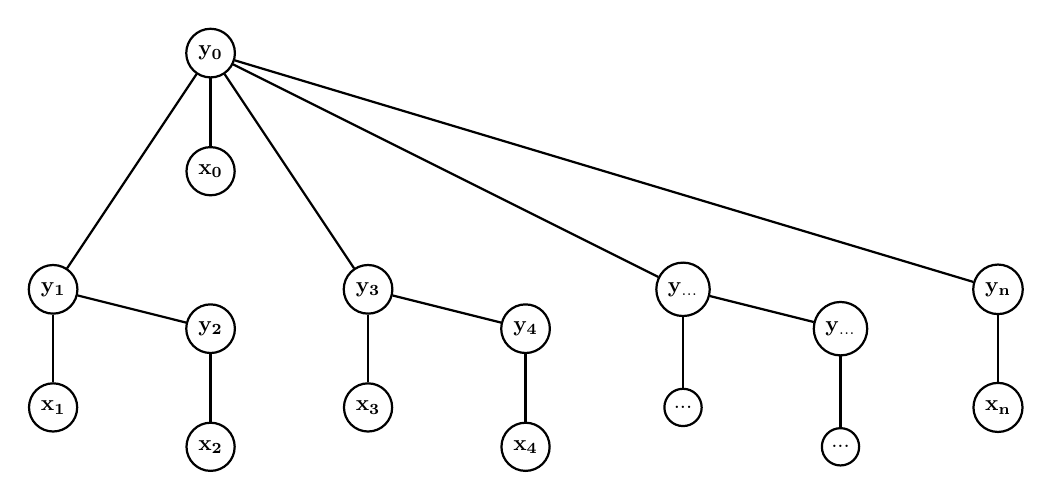
\begin{tikzpicture}[style=thick,scale=1]
            \begin{scope}[shape=circle,minimum size=0.1cm]
            \tikzstyle{every node}=[draw,fill]
            
            \node[fill=none,scale=\nodesize] (y_0) at (2,4.5) {$\mathbf{y_{0}}$};
            \node[fill=none,scale=\nodesize] (X_0) at (2,3) {$\mathbf{x_0}$};
            
            \node[fill=none,scale=\nodesize] (y_1) at (0,1.5) {$\mathbf{y_{1}}$};
            \node[fill=none,scale=\nodesize] (X_1) at (0,0) {$\mathbf{x_1}$};
            \node[fill=none,scale=\nodesize] (y_10) at (2,1.0) {$\mathbf{y_{2}}$};
            \node[fill=none,scale=\nodesize] (X_10) at (2,-0.5) {$\mathbf{x_2}$};
            
            \node[fill=none,scale=\nodesize] (y_2) at (4,1.5) {$\mathbf{y_{3}}$};
            \node[fill=none,scale=\nodesize] (X_2) at (4,0) {$\mathbf{x_3}$};
            \node[fill=none,scale=\nodesize] (y_20) at (6,1.0) {$\mathbf{y_{4}}$};
            \node[fill=none,scale=\nodesize] (X_20) at (6,-0.5) {$\mathbf{x_4}$};
            
            \node[fill=none,scale=\nodesize] (y_3) at (8,1.5) {$\mathbf{y_{\ldots}}$};
            \node[fill=none,scale=\nodesize] (X_3) at (8,0) {$\mathbf{...}$};
            \node[fill=none,scale=\nodesize] (y_30) at (10,1.0) {$\mathbf{y_{\ldots}}$};
            \node[fill=none,scale=\nodesize] (X_30) at (10,-0.5) {$\mathbf{...}$};          
            
            \node[fill=none,scale=\nodesize] (y_4) at (12,1.5) {$\mathbf{y_{n}}$};
            \node[fill=none,scale=\nodesize] (X_4) at (12,0) {$\mathbf{x_n}$};
            
            \draw [-] (X_0) -- (y_0);
            
            \draw [-] (y_0) -- (y_1);
            \draw [-] (X_1) -- (y_1);
            \draw [-] (y_1) -- (y_10);
            \draw [-] (X_10) -- (y_10);
            
            \draw [-] (y_0) -- (y_2);
            \draw [-] (X_2) -- (y_2);
            \draw [-] (y_2) -- (y_20);
            \draw [-] (X_20) -- (y_20);
            
            \draw [-] (y_0) -- (y_3);
            \draw [-] (X_3) -- (y_3);
            \draw [-] (y_3) -- (y_30);
            \draw [-] (X_30) -- (y_30);
            
            \draw [-] (y_0) -- (y_4);
            \draw [-] (X_4) -- (y_4);
            
            \end{scope}
        \end{tikzpicture}
            \caption{Tree structure model}
            \label{fig:tree_graph}
        \end{center}
\end{figure}
\end{small}

\begin{enumerate}
\item[(a)] Write the log likelihood for this model of a single instance $\vx$: $\log{p(\vy,\vx)}$. 

\begin{answertext}{4cm}{}

\end{answertext} 

\item[(b)] Write the conditional log likelihood for this model of a single instance $\vx$: $\log{p(\vy|\vx)}$. 

\begin{answertext}{5cm}{}

\end{answertext} 
\item[(c)] Assume that each variable $y_i$ can take one of $k$ possible states, and variable $x_i$ can take one of $k'$ possible states, where $k'$ is very large. Describe the computational challenges of modeling $\log p(\vy,\vx)$ vs $\log p(\vy|\vx)$.

\begin{answertext}{4cm}{}

\end{answertext} 
\end{enumerate}

{\bf Question 2.} [10 pts]

\begin{enumerate}
\item[(a)] Suppose you wanted to compute $S = \sum^{100}_{x_1 = 1} \dots \sum^{100}_{x_8 = 1} h(x)$ where
\begin{equation*}
    h(x) = \exp(x_1 x_2 + x_4 x_5 + x_7 x_8) \prod_{i=2,5,7} (x_i + x_3 + x_6)^i.
\end{equation*}
It looks like the sum has $100^8 = 10^{16}$ terms, so it seems we must evaluate $h$ $10^{16}$ times. Explain (precisely) how you can compute $S$ with at most $10^7$ evaluations of $h$ or something simpler than $h$.

\begin{answertext}{5cm}{}

\end{answertext} 

\item[(b)] Draw the MRF associated with this distribution.

\begin{answertext}{5cm}{}

\end{answertext} 
\end{enumerate}

\pagebreak

\section*{DAGs, Clique Trees and Message Passing.}

\textbf{Question 3.} [45 pts]
\begin{center}
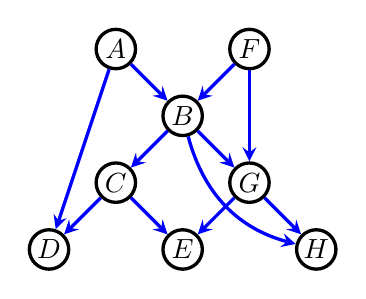
\begin{tikzpicture}[>=stealth, node distance=1.2cm]
    \tikzstyle{format} = [draw, very thick, circle, minimum size=5.0mm,
	inner sep=0pt]

	\begin{scope}
		\path[->, very thick]
			node[format] (A) {$A$}
			node[format, below right of=A] (B) {$B$}
			node[format, below left of=B] (C) {$C$}
			node[format, below left of=C] (D) {$D$}
			node[format, below right of=C] (E) {$E$}
			
			node[format, above right of=B] (F) {$F$}
			node[format, below right of=B] (G) {$G$}
			node[format, below right of=G] (H) {$H$}

			(A) edge[blue] (B)
			(B) edge[blue] (C)

			(C) edge[blue] (D)
			(C) edge[blue] (E)

			(F) edge[blue] (B)
			(B) edge[blue] (G)
			(G) edge[blue] (H)
			
			(A) edge[blue] (D)
			(B) edge[blue,bend right=30] (H)
			(F) edge[blue] (G)
			(G) edge[blue] (E)
		;
	\end{scope}
\end{tikzpicture}
\end{center}

In a statistical DAG model for the graph shown, let ${\bf V} = \{ A, B, C, D, E, F, G, H \}$.
\begin{itemize}
\item[(a)] Answer (and explain your answer) the following d-separation queries:
\begin{align*}
A &\ci F \mid D \\
A &\ci G \mid B,C \\
G &\ci A \mid  B,H,D,E,F \\
F &\ci D \mid A,B \\
C &\ci H \mid B 
\end{align*}
\begin{answertext}{5cm}{}

\end{answertext} 

\item[(b)] Write down the local Markov property of this model.

\begin{answertext}{6cm}{}    

\end{answertext}

\item[(c)] Consider a new graph where we reverse the direction of the edge $B \to G$ to point the other way: $B \gets G$ (and leave the other edges the same).  Does the new graph represent the same model as the old?

Hint: write down the local Markov property for the new graph, and see if all statements in it are implied by d-separation in the original graph.  In general, if local Markov of ${\cal G}_1$ is implied by global Markov of ${\cal G}_2$, and local Markov of ${\cal G}_2$ is implied by global Markov of ${\cal G}_1$, then ${\cal G}_1$ and ${\cal G}_2$ represent the same model.  Otherwise they do not.

\begin{answertext}{5cm}{}

\end{answertext}

\item[(d)] A moralized graph ${\cal G}^a$ is obtained from a DAG ${\cal G}$ by connecting all non-adjacent variables $V_i$ and $V_j$ such
that $V_i \to V_k \gets V_j$ is in the graph (for some $V_k$), and replacing all directed edges by undirected edges.
What is the moralized graph for the DAG in this problem?
\begin{answertext}{7cm}{}

\end{answertext}

\item[(e)] Write down the MRF factorization of the moralized graph ${\cal G}^a$.

\begin{answertext}{3cm}{}    

\end{answertext}

\item[(f)] Is this graph chordal?  If not, add as few edges as possible to make it chordal.  If you added edges, write the factorization of the new graph.

\begin{answertext}{5cm}{}

\end{answertext}
\item[(g)] Create a clique tree from the triangulated graph above (either ${\cal G}^a$ if it is chordal, or the graph obtained from ${\cal G}^a$ by adding new edge(s) to make it chordal).

\begin{answertext}{5.5cm}{}

\end{answertext}

\item[(h)] Pick a root $\vec{R}$ of the clique tree, and calculate both incoming messages $\phi^{\vec{S}_i\to\vec{S}_j}$ from each
$\vec{S}_i$ towards its neighbor $\vec{S}_j$ closer to the root, and outgoing messages $\phi^{\vec{S}_k\gets\vec{S}_i}$ from $\vec{S}_i$ to each neighbor $\vec{S}_k$ further than $\vec{S}_i$ from the root, in terms of clique potentials and other messages.

\begin{answertext}{6cm}{}

\end{answertext}

\item[(i)] By substituting in the clique factors in each message, show that in this example,

for each leaf node $\vec{S}_i$ with a neighbor node $\vec{S}_j$,
{\small
\begin{align*}
p(\vec{S}_i) =
\frac{
\phi^{\vec{S}_i \gets \vec{S}_j}_{\vec{S}_j \setminus \vec{S}_i} \phi_{\vec{S}_i}
}{
\sum_{\vec{S}_i}
\phi^{\vec{S}_i \gets \vec{S}_j}_{\vec{S}_j \setminus \vec{S}_i} \phi_{\vec{S}_i}
}
=
\frac{
\sum_{\vec{V} \setminus \vec{S}_i} \prod_{C \in {\cal C}({\cal G})} \phi_C
}{
\sum_{\vec{V}} \prod_{C \in {\cal C}({\cal G})} \phi_C
}
\end{align*}
}
for each non-leaf note $\vec{S}_i$ with a neighbor $\vec{S}_j$ closer to the root, and neighbors $\vec{S}_1, \ldots, \vec{S}_m$ further from the root that
{\small
\begin{align*}
p(\vec{S}_i) =
\frac{
\phi^{\vec{S}_i \gets \vec{S}_j}_{\vec{S}_j \setminus \vec{S}_i} \phi_{\vec{S}_i}
\left( \prod_{k=1}^m \phi^{\vec{S}_k \to \vec{S}_i}_{\vec{S}_k \setminus \vec{S}_i} \right) \phi_{\vec{S}_i}
}{
\phi^{\vec{S}_i \gets \vec{S}_j}_{\vec{S}_j \setminus \vec{S}_i} \phi_{\vec{S}_i}
\left( \prod_{k=1}^m \phi^{\vec{S}_k \to \vec{S}_i}_{\vec{S}_k \setminus \vec{S}_i} \right) \phi_{\vec{S}_i}
}
=
\frac{
\sum_{\vec{V} \setminus \vec{S}_i} \prod_{C \in {\cal C}({\cal G})} \phi_C
}{
\sum_{\vec{V}} \prod_{C \in {\cal C}({\cal G})} \phi_C
}
\end{align*}
}
and finally for the root node $\vec{S}_i$ with neighbors $\vec{S}_1, \ldots, \vec{S}_m$ that
{\small
\begin{align*}
p(\vec{S}_i) =
\frac{
\left( \prod_{k=1}^m \phi^{\vec{S}_k \to \vec{S}_i}_{\vec{S}_k \setminus \vec{S}_i} \right) \phi_{\vec{S}_i}
}{
\left( \prod_{k=1}^m \phi^{\vec{S}_k \to \vec{S}_i}_{\vec{S}_k \setminus \vec{S}_i} \right) \phi_{\vec{S}_i}
}
=
\frac{
\sum_{\vec{V} \setminus \vec{S}_i} \prod_{C \in {\cal C}({\cal G})} \phi_C
}{
\sum_{\vec{V}} \prod_{C \in {\cal C}({\cal G})} \phi_C
}
\end{align*}
}
\end{itemize}

Here $\vec{V}$ is all variables in the graph, and ${\cal C}({\cal G})$ is the set of maximal cliques in the graph.

\begin{answertext}{15cm}{}

\end{answertext}

\end{document}
